%  LaTeX support: latex@mdpi.com 
%  In case you need support, please attach all files that are necessary for compiling as well as the log file, and specify the details of your LaTeX setup (which operating system and LaTeX version / tools you are using).

%=================================================================
\documentclass[journal,article,submit,moreauthors,pdftex]{Definitions/mdpi} 

\usepackage{enumitem}
\hypersetup{
    colorlinks,
    linkcolor={red!50!black},
    citecolor={blue!50!black},
    urlcolor={blue!80!black},
    pdfborder={0 0 0}
}
\usepackage{hyperref}
\usepackage{multirow}
\usepackage{pgfplots}
\usepackage{float}
\usepackage{amssymb}
\usepackage{cleveref}
\usepackage[english]{babel}
\usepackage[utf8]{inputenc}
% \usepackage[T1]{fontenc}
% \usepackage{changepage}
\usepackage{longtable}
\usepackage{tabularx}
\usepackage{listings}
\lstdefinelanguage[]{spq}
{
    morecomment=[s][\color{olive}\bf]{<}{>},
    basicstyle = \ttfamily\footnotesize,
    commentstyle=\color{green},
    keywordstyle=\color{brown},
    morecomment=[s][\color{blue}\bf]{?}{\ },
    morekeywords={BASE,PREFIX,SELECT,DISTINCT,CONSTRUCT,DESCRIBE,ASK,%
    FROM,NAMED,WHERE,ORDER,BY,ASC,DESC,LIMIT,OFFSET,OPTIONAL,%
    GRAPH,UNION,FILTER,a,STR,LANG,LANGMATCHES,DATATYPE,BOUND,%
    isIRI,isURI,isBLANK,isLITERAL,REGEX,true,false},%
    sensitive=false,%
    % morecomment=[l]\#,%
    morestring=[d][\color{red}]',%
    morestring=[d]"%
}
% \usepackage[showframe=true]{geometry}
%

\newcommand{\textttt}[1] {\texttt{\footnotesize#1}}
\newcommand{\te}[1] {\texttt{\footnotesize#1}}
\newcommand{\h} {\hphantom ~ }
% \newcommand{\textttt}[1] {\mbox{\texttt{\footnotesize#1}}}
% \newcommand{\textttt}[1] {
% \begin{verbatim} #1 \end{verbatim}
% }
\linespread{1}
\pgfplotsset{compat=1.5}
\pgfplotsset
{
	width=0.5\textwidth,
	x tick label style={/pgf/number format/1000 sep=},
  enlarge x limits = 0.0,
  ymajorgrids=true,
	major tick style={draw=none},
  ymin = 0.0,
	every axis/.append style={
		every x tick label/.append style={font=\tiny},
    every y tick label/.append style={font=\tiny},
    every axis label/.append style={font=\small},
    height=37mm,
    width=37mm,
    title style={at={(0.5,0.90)}, font=\normalfont},
    xticklabel style={yshift=4pt}
	}
}
\usepackage{booktabs}
% If you would like to post an early version of this manuscript as a preprint, you may use preprint as the journal and change 'submit' to 'accept'. The document class line would be, e.g., \documentclass[preprints,article,accept,moreauthors,pdftex]{mdpi}. This is especially recommended for submission to arXiv, where line numbers should be removed before posting. For preprints.org, the editorial staff will make this change immediately prior to posting.

%--------------------
% Class Options:
%--------------------
%----------
% journal
%----------
% Choose between the following MDPI journals:
% acoustics, actuators, addictions, admsci, aerospace, agriculture, agriengineering, agronomy, algorithms, animals, antibiotics, antibodies, antioxidants, applsci, arts, asc, asi, atmosphere, atoms, axioms, batteries, bdcc, behavsci , beverages, bioengineering, biology, biomedicines, biomimetics, biomolecules, biosensors, brainsci , buildings, cancers, carbon , catalysts, cells, ceramics, challenges, chemengineering, chemistry, chemosensors, children, cleantechnol, climate, clockssleep, cmd, coatings, colloids, computation, computers, condensedmatter, cosmetics, cryptography, crystals, dairy, data, dentistry, designs , diagnostics, diseases, diversity, drones, econometrics, economies, education, ejihpe, electrochem, electronics, energies, entropy, environments, epigenomes, est, fermentation, fibers, fire, fishes, fluids, foods, forecasting, forests, fractalfract, futureinternet, futurephys, galaxies, games, gastrointestdisord, gels, genealogy, genes, geohazards, geosciences, geriatrics, hazardousmatters, healthcare, heritage, highthroughput, horticulturae, humanities, hydrology, ijerph, ijfs, ijgi, ijms, ijns, ijtpp, informatics, information, infrastructures, inorganics, insects, instruments, inventions, iot, j, jcdd, jcm, jcp, jcs, jdb, jfb, jfmk, jimaging, jintelligence, jlpea, jmmp, jmse, jnt, jof, joitmc, jpm, jrfm, jsan, land, languages, laws, life, literature, logistics, lubricants, machines, magnetochemistry, make, marinedrugs, materials, mathematics, mca, medicina, medicines, medsci, membranes, metabolites, metals, microarrays, micromachines, microorganisms, minerals, modelling, molbank, molecules, mps, mti, nanomaterials, ncrna, neuroglia, nitrogen, notspecified, nutrients, ohbm, optics, particles, pathogens, pharmaceuticals, pharmaceutics, pharmacy, philosophies, photonics, physics, plants, plasma, polymers, polysaccharides, preprints , proceedings, processes, proteomes, psych, publications, quantumrep, quaternary, qubs, reactions, recycling, religions, remotesensing, reports, resources, risks, robotics, safety, sci, scipharm, sensors, separations, sexes, signals, sinusitis, smartcities, sna, societies, socsci, soilsystems, sports, standards, stats, surfaces, surgeries, sustainability, symmetry, systems, technologies, test, toxics, toxins, tropicalmed, universe, urbansci, vaccines, vehicles, vetsci, vibration, viruses, vision, water, wem, wevj

%---------
% article
%---------
% The default type of manuscript is "article", but can be replaced by: 
% abstract, addendum, article, benchmark, book, bookreview, briefreport, casereport, changes, comment, commentary, communication, conceptpaper, conferenceproceedings, correction, conferencereport, expressionofconcern, extendedabstract, meetingreport, creative, datadescriptor, discussion, editorial, essay, erratum, hypothesis, interestingimages, letter, meetingreport, newbookreceived, obituary, opinion, projectreport, reply, retraction, review, perspective, protocol, shortnote, supfile, technicalnote, viewpoint
% supfile = supplementary materials

%----------
% submit
%----------
% The class option "submit" will be changed to "accept" by the Editorial Office when the paper is accepted. This will only make changes to the frontpage (e.g., the logo of the journal will get visible), the headings, and the copyright information. Also, line numbering will be removed. Journal info and pagination for accepted papers will also be assigned by the Editorial Office.

%------------------
% moreauthors
%------------------
% If there is only one author the class option oneauthor should be used. Otherwise use the class option moreauthors.

%---------
% pdftex
%---------
% The option pdftex is for use with pdfLaTeX. If eps figures are used, remove the option pdftex and use LaTeX and dvi2pdf.

%=================================================================
\firstpage{1} 
\makeatletter 
\setcounter{page}{\@firstpage} 
\makeatother
\pubvolume{xx}
\issuenum{1}
\articlenumber{5}
\pubyear{2019}
\copyrightyear{2019}
%\externaleditor{Academic Editor: name}
\history{Received: date; Accepted: date; Published: date}
%\updates{yes} % If there is an update available, un-comment this line

%% MDPI internal command: uncomment if new journal that already uses continuous page numbers 
%\continuouspages{yes}

%------------------------------------------------------------------
% The following line should be uncommented if the LaTeX file is uploaded to arXiv.org
%\pdfoutput=1

%=================================================================
% Add packages and commands here. The following packages are loaded in our class file: fontenc, calc, indentfirst, fancyhdr, graphicx, lastpage, ifthen, lineno, float, amsmath, setspace, enumitem, mathpazo, booktabs, titlesec, etoolbox, amsthm, hyphenat, natbib, hyperref, footmisc, geometry, caption, url, mdframed, tabto, soul, multirow, microtype, tikz

%=================================================================
%% Please use the following mathematics environments: Theorem, Lemma, Corollary, Proposition, Characterization, Property, Problem, Example, ExamplesandDefinitions, Hypothesis, Remark, Definition, Notation, Assumption
%% For proofs, please use the proof environment (the amsthm package is loaded by the MDPI class).

%=================================================================
% Full title of the paper (Capitalized)
\Title{A Linked Open Social Dataset for Scientific Benchmarking}

% Author Orchid ID: enter ID or remove command
\newcommand{\orcidauthorA}{https://orcid.org/0000-0002-9699-629X} % Add \orcidA{} behind the author's name
\newcommand{\orcidauthorB}{https://orcid.org/0000-0002-5399-5860} % Add \orcidB{} behind the author's name

% Authors, for the paper (add full first names)
\Author{Renato Fabbri $^{1}$*\orcidA{} and Osvaldo N. Oliveira Junior $^{2}$\orcidB{}}

% Authors, for metadata in PDF
\AuthorNames{Renato Fabbri, Osvaldo Novais de Oliveira Junior}

% Affiliations / Addresses (Add [1] after \address if there is only one affiliation.)
\address{%
$^{1}$ \quad Institute of Mathematical and Computer Sciences, University of São Paulo (ICMC/USP), São Carlos, Brazil; renato.fabbri@gmail.com\\
$^{2}$ \quad São Carlos Institute of Physics, University of São Paulo (IFSC/USP), São Carlos, Brazil; chu@ifsc.usp.br}

% Contact information of the corresponding author
\corres{Correspondence: renato.fabbri@gmail.com}

% Current address and/or shared authorship
% \firstnote{Current address: Affiliation 3} 
% \secondnote{These authors contributed equally to this work.}
% The commands \thirdnote{} till \eighthnote{} are available for further notes

%\simplesumm{} % Simple summary

%\conference{} % An extended version of a conference paper

% Abstract (Do not insert blank lines, i.e. \\) 
\abstract{
The fields of social network analysis and complex networks
are widely researched.
In fact, a myriad of results have been reported which are based in
diverse data, most often not accessible to researchers other than the publishing authors.
In order to furnish the scientific community with a common repertoire,
this work presents an open dataset with diverse provenance of 
human social online networking.
Current data was obtained in 2013-16 from well-known online social networking platforms:
Facebook, Twitter, IRC, Email.
Data from ParticipaBR, AA, and Cidade Democrática are also supplied as samples of less known instances.
The linked data representation was adopted in order to
comply with current best practices, homogenize access, facilitate discovery
and analyzes which integrate third party and provided instances.
Futhermore, the method for obtaing and making the data available is potentially novel, and may of use for other research groups.
This document presents a description, usage remarks and overall statistics of the dataset, which should favor subsequent work in complex and social networks
  and enhancements to the dataset.
}

% Keywords
\keyword{social networks; complex networks; linked data; semantic web; big data; benchmark data; Facebook; Twitter; irc; email}

%%%%%%%%%%%%%%%%%%%%%%%%%%%%%%%%%%%%%%%%%%
% Only for the journal Data:
\dataset{https://rfabbri.linked.data.world/d/linked-open-social-data/}

\datasetlicense{CC0}

\begin{document}
\section{Summary}
The research on human social and complex networks often rely on data that express real phenomena~\cite{c1,c2,c3}.
Such data is regularly not made publicly available,
which hinders validation of the results
and does not favor subsequent work.
Furthermore, there is a lack of open datasets for benchmarking results
related to complex and social networks,
yielding diverse results from poorly related sources.
Social networks linked data is currently scarce and not stable
or rigorous enough to be a public reference on statistical physics
and social networks research~\cite{l1,l2}.

This work presents a collection of linked and open data
derived from online human social networks.
The dataset is named LOSD (Linked Open Social Data),
and has been achieved by linking social data into a dataset derived from diverse
provenance, namely: Facebook, Twitter, IRC, Email groups, ParticipaBR, Cidade Democrática, and AA.
Such data is proposed as a common and public repertoire for scientific
research involving networks and textual content.
In fact, the data has already been used in scientific research~\cite{stab,thesis} (CNPq grant ), and should be used in further research in complex networks and data visualization (FAPESP grant ) which relies on networks enriched by textual data and on dynamic (or time-evolving) networks.


\subsection{Related work}
Most available datasets on human social networks rely on only one source~\cite{o1,o2,o3,o4},
on specialized communities such as related to research and movies~\cite{s1,s2,s3,s4,s5},
or present only statistics about social networks, and not the data that yields the networks~\cite{st1,st2,st3,st4}.
Contributions which are most similar to LOSD are mentioned in this section.
In~\cite{fb1}, data obtained only from Facebook is reported.
With such a focus, the authors made available a number of statistics,
but the data is offline at least since 2010.
Linked human social network data is scarcely found in the scientific community.
In~\cite{foaf1}, the authors presented a set of tools to obtain linked social data available in the public data cloud, and made available a dataset from the Advogato platform,
dedicated to free software developers linked by trust relatioships.
There are various datasets which makes available data obtained from Twitter (e.g.~\cite{tw1,tw2,t3,t4}),
most often with a specific focus (users, tweets, hashtags, etc)
and not presented to the scientific community by means of a research article.
In summary, no human social network dataset presented to the
scientific community containts the diverse provenance used in LOSD,
potentially because researchers did not have the means to acquire and
share the data as described in Section~\ref{acq}.

\section{Data Description}\label{materials}
\subsection{Data outline}
The database consists of 34,120,026 triples, 3,172,927 network links yield by selected interactions or relations, 382,568 participants and 253,155,020 characters in text data. Among all snapshots, 63 are ego snapshots, 54 are group snapshots; 49 have network interaction links, 89 have network friendship links; 43 have text content from messages.



\begin{table*}[h!]
\begin{center}
\caption{Number of snapshots from each provenance. Every snapshot is a \texttt{po:Snapshot}; there are three types of the \texttt{po:AASnapshot} class.}
\begin{tabular}{| l | c |}\hline
\textbf{snapshot provenance} & \textbf{number of snapshots} \\\hline\hline\hline
http://purl.org/socialparticipation/po/Snapshot & 117 \\\hline
\end{tabular}\end{center}
\end{table*}
\label{outline}
Current overall results concern data selection and preparation for data discovery.
The main result is the data made available, which enables benchmarking of scientific results
and easy experimentations, and no compliant dataset was found by the authors.
Secondary results include data outline through figures and tables,
software support and example SparQL queries.

\subsection{Standardization}
The data is embedded into URIs and triples, i.e. translated to RDF.
URIs are built in the namespace \url{http://purl.org/socialparticipation/participationontology/}
which are identified herein with the prefix ``\textttt{po:}''.
Classes and properties are built by adding a suffix to the root, as in \textttt{po:Participant} or \textttt{po:text}.
Classes have ``UpperCamelCase'' suffixes while properties have ``lowerCamelCase'' suffixes.
All class instances, such as participants, messages, friendships and
interactions, are linked to
snapshots through the triple \textttt{<instance> po:snapshot <snapshot\_uri>}.
Message texts, including comments, are objects in the triple: \textttt{<message\_id> po:text <message\_text>}.
Preprocessed texts are objects of triples: \textttt{<message\_id> po:cleanText <message\_text>}.
More specialized predicates are used for delivering text when necessary,
such as \textttt{po:htmlBodyText} and \textttt{po:cleanBodyText} used
for ParticipaBR articles.
A participant URI is unique throughout the provenance (e.g. the same for
the same participant in all Twitter snapshots).
To enable annotations which differ when the snapshot changes,
\texttt{po:Observation} class instances are used in the triple
\textttt{<participant\_uri> po:observation <observation\_uri>}.
The observation instances are then linked to the snapshot and the
data.

Instance URIs are built using the URI from the class they derive from plus a hashtag character,
a provenance string (e.g. \textttt{facebook-legacy} or
\textttt{participabr-legacy}), and an identifier;
i.e. \textttt{po:Participant\#<provenance-legacy>-<id>}.
All snapshot URIs follow the formation rule: \textttt{po:<SnapshotProvenance>\#<snapshot\_id>}.
All snapshot ids follow the formation rule: \textttt{<platform>-legacy-<further\_identifier>}; e.g.
\textttt{irc-legacy-labmacambira} or
\textttt{email-legacy-linux.audio.devel1-20000}.

Data was gathered from:
\begin{itemize}
    \item public APIs (Twitter, Email);
    \item public logs (IRC and AA);
    \item Netvizz software~\cite{netvizz} and subsequent donation by users (Facebook);
    \item donation by system administrators (AA, ParticipaBR, Cidade Democr\'atica).
\end{itemize}

Integration and uniformity of access is obtained through linked data
representation, as described in Section~\ref{queries}.
This section introduces the underlying data in very concise terms.
One should access the Supporting Information document for
a more information about the dataset.

\subsection{Snapshots}
Of central importance to presented database is the concept of a snapshot.
A snapshot is herein a set of data gathered together, at a contiguous time
unit.
Examples: the first 20 thousand email messages of an email list
comprises a snapshot; the tweets from the MAMA music event is a
snapshot; the friendship, interaction and posts structures of a facebook
group, prospected at the same time, is a snapshot.

\subsection{Facebook data}
Friendship ego networks (networks whose nodes represent friends of a user)
were donated from individual users in 2013 and 2014.
Friendship and interaction networks from groups were gathered from
groups where the first author was a participant.
Additionally, some groups have post texts along some metadata, such as
the number of likes.

\subsection{Twitter data}
Tweets were gathered through the Twitter streaming public API.
Each snapshot is unified by a distinct hashtag.
Network links are canonically yield by retweets,
but replies and user mentions are also kept in the database.

\subsection{IRC data}
Public IRC (Internet Relay Chat) logs were used to obtain IRC snapshots.
The database has records of relations yield by directed messages and
mentions.

\subsection{Email data}
Email snapshots refer to individual email lists.
All messages were obtained from the Gmane public email archive~\cite{gmane}.
Each message has the original text and the text without some of the lines
from previous messages or that are software code or author signature.
Most importantly, each message instance holds the ID of the message it is
a reply to, if any, which enables the achievement of interaction networks~\cite{bird,stab}

\subsection{ParticipaBR data}
ParticipaBR was a Brazilian federal platform for social participation,
the most important platform from the myriad of social participation platforms
that were available in 2011-2018~\cite{spbr}.
Texts are derived from blog posts and networks may be obtained from
friendship and interaction criteria.

\subsection{Cidade Democr\'atica data}
Cidade Democrática is a Brazilian civil society social participation portal.
Data gathered is complex in the number of types of instances.

\subsection{AA data}
AA (Algorithmic Autoregulation~\cite{aa,aa2}) is a software to keep track of dedications,
it is based on testifying and sharing ongoing work.
The data was gathered from different versions of the system and from an IRC
log.
 
 
%%%%%%%%%%%%%%%%%%%%%%%%%%%%%%%%%%%%%%%%%%
\section{Methods}
LOSD is expressed as linked data through RDF
and is ontologicaly described through the
data-driven ontology synthesis method presented in Section~\ref{ont}.

\subsection{Data acquisition}\label{acq}
Research involving human subjects raise well-known ethic issues~\cite{}.
Furthermore, the online social networking platforms often restrict access
to the data and declare illegal the use of their data through web crowlers~\cite{ile1,ile2}.
In this context, research using data, e.g. from Facebook, is considered
problematic if not prohibited.
We reached a potential solution to this issue through continuated research with
collaborators in the fields of phylosophy, social sciences, and psychology.
The conceptual framework is presented in~\cite{antphy,antphy2}, and in essence
consists in researching first the social networks related to the researchers,
and keeping the procedures, data, algorithms and results publicly available.
This practices enabled collecting and sharing the data in LOSD.
Notice that, although Twitter data is available through public APIs, the other sources are more problematic.

% download via netviz when fb allowed it, donations
% twitter, bots, gmane
% contact with developers of AA, PBR, CD
% Anthropological physics

\subsection{Linked open data}
Linked data refers to data published in the web in such a way that it is
machine readable and conforms to a set of best practices.
The yielded web of data is composed of documents on the web
such as the web of HTML documents.
In practice, the publication of linked data can me summarized
by 1) the use of RDF to publish data on the web and 2) the use of RDF
links to interlink data from different sources~\cite{ld1,ld2}.
The web is expected to be interconnected and to grow by the systematic application of four
steps~\cite{lee1}:
\begin{itemize}
    \item Use URIs to identify things~\cite{uri}.
    \item Use HTTP URIs.
    \item Provide useful information when a URI is accessed via HTTP.
    \item Provide other URIs in the description of resources so human
        and machine agents can perform discovery.
\end{itemize}

The Linked Open Data~\cite{lod} is a constantly growing cloud of data,
the global data space, which is usually
conceived as centered around the DBPedia, a linked data representation
of data from Wikipedia~\cite{dbpedia0,dbpedia},
and sometimes called the Giant Global Graph (GGG, akin to the WWW).

\subsection{RDF}
The Resource Description Framework (RDF), a W3C
recommendation, is a model for data
interchange~\cite{w3cr}.
It is based on the idea of making statements about resources in the form
of triples, i.e. expressions in the form ``subject - predicate -
object''.
RDF can be serialized in several file formats, including RDF/XML,
Turtle and Manchester, which all, in essence, represent a labeled and
directed multi-graph.
RDF may be stored in a type of database called a triplestore~\cite{rdf}.

As an example of an RDF statement, the following triple in the Turtle
format asserts that ``the paper has color white'':\\
\texttt{http://example.org/Thing\#Paper http://example.org/hasColor\\
http://example.org/Color\#White .}

\subsection{RDFS and OWL ontologies}\label{sont}
One of the most important notions of the semantic web is that of an ontology~\cite{ont}.
An ontology, in this context, is a formalized conceptualization, comprised by
concepts and relations between the concepts and between the relations themselves.
In current semantic web, most simple ontologies are written using the RDFS protocol,
by which one can specify, among other things~\cite{rdfs}:
\begin{itemize}
  \item concepts;
  \item properties, which are concepts that are used as predicates and thus relate concepts;
  \item special relations between concepts that state that one concept is more general than the other\footnote{This
          kind of relation is called hypernymy. Examples: mammal is a hypernym of monkey, drink is a hypernym of beer.};
  \item the subjects and objects that can occurs in a triple where a specific property is a predicate.
\end{itemize}

One can also write an ontology using the OWL protocol,
with which all the expressive capabilities of RDFS are
available, but one can also, among other things~\cite{owl}:
\begin{itemize}
  \item state ``property axioms'', i.e. specify if a property is e.g. reflexive or transitive;
  \item state ``class restrictions'', i.e. specify if a class instance e.g. necessarily holds a relation to another class instance or data.
\end{itemize}
OWL has a richer vocabulary than RDFS and is (way more) complex.
This complexity is a drawback together with the greater computational cost
for performing inference.
The advantage is the greater power to represent conceptualizations.
Using ontologies enables automated reasoning.
For example, if a property \textttt{:r} is known to relate only mokeys to trees,
then, if there is a triple \textttt{:a :r :b}, the instance \textttt{:a} is considered a monkey,
and instance \textttt{:b} is considered a tree,
even if there is no explicit declaration similar
to \textttt{:a rdf:type :Mokey}.

For the data described in this article, the following features are most relevant~\cite{rdfs,owl}:
\begin{itemize}
  \item Using RDFS, one may define a property domain, i.e. the class instances that are allowed as the object in a triple with the property.
  \item Using RDFS, one may define a property range, i.e. the class instances that are allowed as the predicate in a triple with the property.
  \item Using OWL, one may define an existential restriction for a class \textttt{:C},
    i.e. declare that an instance \textttt{:C\#I} of such class has at least one relation with a property \textttt{:p} and a class \textttt{:C2} in the form
    \textttt{:C\#I :p :C2\#I}, where \textttt{:C2\#I} is an instance of the class \textttt{:C2}.
  \item Using OWL, one may define an universal restriction for a class \textttt{:C},
    i.e. declare that any relation of an instance \textttt{:C\#I} of such class, with a property \textttt{:p} of the form \textttt{:C\#I :p :CX\#I},
    implies that \textttt{:CX\#I} is an instance of a specific class, e.g. \textttt{:C2}.
\end{itemize}


\subsection{Data-driven ontology synthesis}\label{ont}
OWL Ontologies are tools to describe taxonomies and the
structure of knowledge~\cite{owl1}.
Most ontologies are created by domain experts even though the data they
arrange is often given by a software system and has a predefined
structure~\cite{owl2}. 

We developed a simple ontology synthesis method that probes
the ontological structure in the data with
SPARQL queries and post-processing.
The results are OWL code and diagrams which are available in the
Supporting Information document of this article.
The method can be extended to comprise further OWL axioms and restrictions,
but is currently performed to fit present needs with maximum simplicity.
Present needs are limited to informative figures and
the steps implemented are as follows:
\begin{enumerate}[leftmargin=0cm]
    \item Obtain all distinct classes with the query:\\
        \h\textttt{SELECT DISTINCT ?class\_uri WHERE \{ ?s a ?class\_uri .\}}
\item For each class, obtain the properties that occur as predicates in triples where the subject is an instance of the class:\\
	\h\textttt{SELECT DISTINCT ?property\_uri WHERE \{ ?s a <class\_uri> . ?s ?property\_uri ?o .\}}\\
Such properties are used to assert existential and universal restrictions for the class.
\item Compare the total number of individuals (\textttt{?cs1}) of the class (\textttt{class\_uri}) with
	the number of such individuals (\textttt{?cs2}) that are subjects of at least one triple where 
        the predicate is the property (\textttt{property\_uri}) and the object is
        an instance of the same class (\textttt{class2\_uri}).
	The queries are:\\
	\h\textttt{SELECT (COUNT(DISTINCT ?s) as ?cs1) WHERE \{ ?s a <class\_uri> \}}\\
        \h\textttt{SELECT DISTINCT ?oc WHERE \{\\
	\h\h ?s a <class\_uri>. ?s <property\_uri> ?o . ?o a ?oc . \\ 
        \h\}}\\
        Then, for each object class (\textttt{object\_curi}) in \textttt{?oc}:\\
	\h\textttt{SELECT (COUNT(DISTINCT ?s) as ?cs2) WHERE \{\\
	\h\h ?s a <class\_uri>. ?s <property\_uri> ?o . ?o a <object\_curi> .\\         \h\}}\\
        When \textttt{?cs1} matches \textttt{?cs2}, an existential restriction is found. And with the query:
	\h\textttt{SELECT (COUNT(DISTINCT ?s) as ?cs) WHERE \{\\
	\h\h ?s a <class\_uri> . ?s <property\_uri> ?o . ?o a ?oc .\\
        \h\h FILTER(str(?oc) != 'object\_curi')\\
        \h\}}\\
       When \textttt{?cs} is 0, a universal restriction is found. 
\item To keep a record of further restrictions, get all object classes or datatypes where the subject is an instance of the class and the predicate is the property:\\
	\h\textttt{SELECT DISTINCT ?co (datatype(?o) as ?do) WHERE \{\\
        \h\h ?s a <class\_uri>. ?s <property\_uri> ?o . OPTIONAL \{ ?o a ?co . \}\\
        \h\}}
    \item Obtain all distinct properties:\\
        \h\textttt{SELECT DISTINCT ?p WHERE \{ ?s ?p ?o \}}
    \item Check if each property is functional, i.e. if it
        occurs at most once with each subject.
        This is performed by counting the objects and further verifying
        that they are at most one. The query is:\\
        \h\textttt{SELECT DISTINCT (COUNT(?o) as ?co) WHERE \{ ?s
            <property\_uri> ?o \} GROUP BY ?s}
          \item For each property, find the incident range (possible subjects) and domain (possible objects) with the
        queries:\\
        \h\textttt{SELECT DISTINCT ?co (datatype(?o) as ?do) WHERE \{\\
        \h\h ?s <property\_uri> ?o . OPTIONAL \{ ?o a ?co . \}\\
        \h\}} \\
        and \\
        \h\textttt{SELECT DISTINCT ?cs WHERE \{ ?s <property\_uri> ?o . ?s a ?cs . \}}
%     \item For each instance of each class, get all distinct predicates.
%         For each predicate, check if all instances of the class
%         hold such relationship (existential restriction):\\
%         \textttt{SELECT DISTINCT ?p WHERE \{ ?s a <class\_uri>. ?s ?p ?o . \}}\\
%         \textttt{SELECT DISTINCT ?s WHERE \{ ?s a <class\_uri> \}}\\
%         \textttt{SELECT DISTINCT ?s ?co  (datatype(?o) as ?do) WHERE \{?s
%                 a <class\_uri>. ?s <property\_uri> ?o . OPTIONAL \{?o a ?co . \}\}}
%     \item and if all instances that hold such relationship are instances of the class
%         (universal restriction):\\
%         \textttt{SELECT DISTINCT ?s WHERE \{ ?s <property\_uri> ?o . \}}
%     \item Draw each class, each property and the overall figure.
      \item Render diagrams to achieve figures as exemplified in Section~\ref{sdia} and in the Supporting Information document.
%      \item Make \textttt{rdfs:subClassOf} and \texttt{rdfs:subPropertyOf}
%          statements to better organize knowledge and link to third party
%          ontologies and data. This step is left aside in current LOSD as 
\end{enumerate}



\section{Usage notes}
%%%%%%%%%%%%%%%%%%%%%%%%%%%%%%%%%%%%%%%%%%
\vspace{6pt} 
\subsection{Software tools}
The authors made available software for rendering analyses and
the data set itself.
\subsubsection{Triplification routines}
For each social platform there is a \emph{triplification} routine,
i.e. a script for expressinf the data as RDF.
Original formats and further observations are presented in
Table~\ref{tab:provenance}.
  {\renewcommand{\arraystretch}{1.2}
\begin{table*}[h!]\scriptsize
\begin{center}
\caption{Social platforms, original formats and further observations for
the database.}\label{tab:provenance}
\begin{tabular}{ l | p{3cm} p{3cm} c }
    \textbf{social platform} & \textbf{original format} & \textbf{further observations} & \textbf{toolbox} \\\specialrule{1.5pt}{1pt}{1pt}
    AA & MySQL and MongoDB databases; IRC text logs & donated by AA users & Participation~\cite{participation} \\\hline
    Cidade Democrática & MySQL database & donated by admins & Participation \\\hline
    Email & mbox & obtained through the Gmane public archive & Gmane~\cite{gmane} \\\hline
    Facebook & GDF, GML and TAB & obtained through Netvizz~\cite{netvizz} & Social~\cite{social} \\\hline
    IRC & plain text log & obtained through Supybot logging & Social \\\hline
    ParticipaBR & PostgreSQL database & donated by admins & Participation \\\hline
    Twitter & JSON & obtained through Twitter streaming API & Social \\
\end{tabular}\end{center}
\end{table*}                    
  }
\subsubsection{Topological and textual analysis}\label{ana}
Routines are available for taking topological and textual measures from
the LOSD data.
  Auxiliary routines, such as for performing principal component analysis (PCA)
  and obtaining statistics derived from the Kolmogorov-Smirnov test~\cite{kol}, are available to ease pattern recognition.

% \subsubsection{Multimedia rendering}\label{media}
% It is a core purpose of framework to provide routines for rendering
% audiovisualizations of the data.
% Social structures are rendered into music, images and video animations
% through the Percolation toolbox~\cite{percolation} in association with
% the Music and Visuals toolboxes~\cite{music,visuals}.

% \subsubsection{Migration from deprecated toolboxes}
% Routines mentioned in Sections~\ref{ana} and~\ref{media} are being migrated from deprecated
% toolboxes~\cite{gmaneLegacy,percolationLegacy} into newly designed
% toolboxes~\cite{percolation,visuals}. TTM, recover?

\subsection{Diagrams of the data and auxiliary tables}\label{sdia}
LOSD navigation may be assisted through diagrams which describes
the structure from each provenance.
Such diagrams are in the Supporting Information document
together with tables to facilitate the appreciation of the provided data.
A very simple example is given in Figure~\ref{dia} where the friendship
structure of the Facebook snapshots is revealed.

\begin{figure}[!ht]
    \centering
    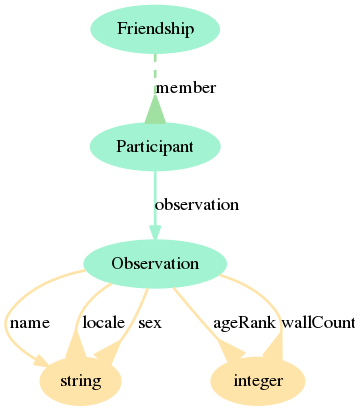
\includegraphics[width=0.5\textwidth]{../ontologies/facebook-legacy-AntonioAnzoategui18022013Friendship.ttl/draw}
    \caption{A diagram of the core structure that entails the friendship networks
    of the Facebook snapshots. A green edge denotes an OWL existential class restriction; an inverted nip denotes an OWL universal class restriction; a full (non-dashed) edge denotes an OWL functional property axiom (see Section~\ref{sont}). Further information and complete diagrams for each provenance are available in the Supporting Information document.}\label{dia}
\end{figure}

\subsection{SPARQL queries}\label{queries}
There are numerous useful and general purpose SPARQL queries to be performed against LOSD.
In this section, a selection of some of the most basic queries are made available due to their potential to be varied.
All queries assume the preamble \textttt{PREFIX po: <http://purl.org/socialparticipation/po/>}.
\begin{enumerate}[leftmargin=0cm]
	\item Retrieve the number of participants:\\
            \h\textttt{SELECT (COUNT(DISTINCT ?author) as ?c) WHERE \{
            ?author a po:Participant . \} }
	\item Retrieve the number of relations, be them interactions or
            friendships:\\
            \h\textttt{SELECT (COUNT(?interaction) as ?c) WHERE \{\\
            \h        \h \{ ?interaction a po:Friendship \} UNION \{ ?interaction
                    a po:Interaction \}\\
            \h        \h  UNION \{ ?interaction po:retweetOf
                    ?message \} \\
            \h\h  UNION \{ ?interaction po:replyTo ?message \}\\
            \h        \h UNION \{ ?interaction po:directedTo ?participant
                    \}\\
            \h\} }
                  \item Retrieve all text produced by a specific user with URI \textttt{user\_uri}:\\
            \h\textttt{SELECT (CONCAT(?text) as ?texts) WHERE \{\\
            \h        \h ?activity po:author <user\_uri> . ?activity po:text ?text .\\
            \h\}}
        \item List 1000 users (URIs and names) with the most friendships and the number of
            friendships in descending order by the number of friendships:\\
            \h\textttt{SELECT DISTINCT ?participant (COUNT(?friendship) as ?c) WHERE \{\\
            \h    \h ?friendship a po:Friendship . ?friendship po:member ?participant . \\
            \h\} ORDER BY DESC(?c) LIMIT 1000}
        \item Retrieve text messages with the word ``crucial'' (case insensitive):\\
            \h\textttt{SELECT ?text WHERE \{ \\
            \h        \h ?activity po:text ?text . FILTER regex(?text, 'crucial', 'i')\\
            \h\}}
\item List participants and respective full names whose name has the substring ``Amanda'':\\
    \h\textttt{SELECT DISTINCT ?participant ?name WHERE \{\\
    \h\h ?participant po:observation ?obs . ?obs po:name ?name .\\
    \h\h FILTER regex(?name, 'Amanda', 'i') \\
    \h\}}
  \item Return all pairs of friends of a participant (with URI \textttt{participant\_uri}) which are friends themselves:\\
     \h\textttt{SELECT DISTINCT ?friend1 ?friend2 WHERE \{\\
     \h\h       ?friendship1 po:member <participant\_uri> . ?friendship1 po:member ?friend1 .\\
     \h\h       ?friendship2 po:member <participant\_uri> . ?friendship2 po:member ?friend2 .\\
     \h\h       ?friendship3 po:member ?friend1 . ?friendship3 po:member ?friend2 .\\
     \h\}}
\item Return all interactions from replies in a snapshot:\\
    \h\textttt{SELECT ?from ?to WHERE \{\\
    \h      \h  ?message1 po:snapshot <snapshot\_uri> .  ?message2 po:replyTo ?message1 .\\
    \h      \h  ?message1 po:author ?from .  ?message2 po:author ?to .\\
    \h\}}
\end{enumerate}

\subsubsection{Obtaining the networks}\label{snet}
A complex network $N=(n,l,m)$ may be regarded essentially as
a set of nodes $n$, a set of links $l$ that related the nodes,
and metadata $m$ such as node and link weights, text related to the nodes, etc.
This section presents the queries for obtaining networks using LOSD
which are promptly envisioned by the authors.
Many other networks may be obtained because the criteria that entail
links, and restrains in the set of nodes and of links,
are determined by the research being developed.
Furthermore, we do not focus here on multilayer networks (e.g. bipartite networks), or on multigraphs (or muldimensional networks), i.e. on networks with more than one type of node or of link.
Here is a list with short descriptions of the networks and the corresponding SPARQL queries:
\begin{itemize}
  \item Overall facebook friendship network available in LOSD:
\begin{lstlisting}[language=spq]
SELECT ?a1 ?a2 WHERE { 
  ?f a po:Friendship .  ?f po:member ?a1 . ?f po:member ?a2 .
}
\end{lstlisting}\vspace{-0.2cm}
  \item Overall facebook friendship network derived only from ego networks:
\begin{lstlisting}[language=spq]
SELECT ?a1 ?a2 WHERE { 
  ?f a po:Friendship . ?f po:snapshot ?s . ?s po:isEgo True .
  ?f po:member ?a1 . ?f po:member ?a2 .

}
\end{lstlisting}\vspace{-0.2cm}
  \item Overall facebook interaction network available in LOSD:
\begin{lstlisting}[language=spq]
SELECT ?a1 ?a2 WHERE { 
  ?f a po:Interaction .
  ?f po:interactionFrom ?a1 . ?f po:interactionTo ?a2 .
}
\end{lstlisting}\vspace{-0.2cm}
  \item Email interaction network for email list shapshot with URI \verb|http://xxxx|, with the all (preliminarily cleaned) text related to each message (node atribute):
\begin{lstlisting}[language=spq]
SELECT ?a1 ?a2 ?t1 ?t2 WHERE { 
  ?m po:snapshot <http://xxxx> . ?m a po:EmailMessage .
  ?m po:author ?a1 . ?m po:replyTo ?m2 . ?m2 po:author ?a2 .
  ?m po:cleanText ?t1 . ?m2 po:cleanText ?t2 .
}
\end{lstlisting}\vspace{-0.2cm}
  \item IRC users related by messages directed to each other, and the text of each message (link attribute):
\begin{lstlisting}[language=spq]
SELECT ?a1 ?a2 ?t WHERE { 
  ?m a po:IRCMessage .  ?m po:author ?a1 . ?m po:directedTo ?a2 .
  ?m po:cleanText ?t .
}
\end{lstlisting}\vspace{-0.2cm}
  \item Twitter users related by retweets:
\begin{lstlisting}[language=spq]
SELECT ?a1 ?a2 WHERE { 
  ?m1 po:retweetOf ?m2 . ?m1 po:author ?a1 . ?m2 po:author ?a2 .
}
\end{lstlisting}\vspace{-0.2cm}
  \item Twitter users related by user mentions and the text of the tweets:
\begin{lstlisting}[language=spq]
SELECT ?a1 ?a2 ?t WHERE { 
  ?m a po:Tweet . ?m po:author ?a1 . ?m po:userMention ?a2 .
  ?m po:text ?t .
}
\end{lstlisting}\vspace{-0.2cm}
  \item Friendship network from ParticipaBR, with the date when each frienship was established:
\begin{lstlisting}[language=spq]
SELECT ?a1 ?a2 ?d WHERE { 
  ?s po:shapshotID 'participabr-legacy' . ?f po:snapshot ?s .
  ?f a po:Friendship . 
  ?f po:member ?a1 . ?f po:member ?a2 . ?f po:createdAt ?d .
}
\end{lstlisting}\vspace{-0.2cm}
  \item Interaction network from ParticipaBR obtained by comments on articles:
\begin{lstlisting}[language=spq]
SELECT ?a1 ?a2 WHERE { 
  ?s po:shapshotID 'participabr-legacy' . ?a po:snapshot ?s .
  ?a a po:Article .
  ?a po:author ?a1 . ?c po:article ?a . ?c po:author ?a2 .
}
\end{lstlisting}\vspace{-0.2cm}
  \item Interaction network from ParticipaBR obtained by comments and votes on comments:
\begin{lstlisting}[language=spq]
SELECT ?a1 ?a2 WHERE { 
  ?s po:shapshotID 'participabr-legacy' . ?c po:snapshot ?s .
  ?c a po:Comment .  ?c po:author ?a1 .
  { ?v a po:Vote . ?v po:reference ?c . ?v po:author ?a2 .
  } UNION {
    ?c2 a po:Comment . ?c2 po:replyTo ?c . ?c2 po:author ?a2 .
  }
}
\end{lstlisting}\vspace{-0.2cm}
  \item Interaction network from Cidade Democrática obtained by comments on Topics:
\begin{lstlisting}[language=spq]
SELECT ?a1 ?a2 WHERE { 
  ?s po:shapshotID 'cidadedemocratica-legacy' . ?t po:snapshot ?s .
  ?t a po:Topic .  ?t po:author ?a1 .
  ?c a po:Comment . ?c po:topic ?t . ?c po:author ?a2 .
}
\end{lstlisting}\vspace{-0.2cm}
  \item AA users, related by AA session validations:
\begin{lstlisting}[language=spq]
SELECT ?a1 ?a2 WHERE { 
  ?s po:author ?a1 . ?s po:checkParticipant ?a2 .
}
\end{lstlisting}\vspace{-0.2cm}
\end{itemize}

Again, this is not an exaustive list.
For example, other instances which are related in LOSD, and have authors,
also yield valid criteria for interaciton networks.
For a less canonical example for obtaining networks, links may be derived from sufficiently similar vocabulary used by participants, or from activity is sufficiently similar dates, which yield networks which are not interaction or friendship networks.
% mk figure with two participants and their relation though response, retweet, or friendship TTM

\section{Conclusions and further work}
\label{conclusions}
This article outlines LOSD, a large human online social networking dataset (with almost 35 million triples) with diverse provenance.
Tools and procedures used to achieve LOSD, and fundamental queries needed to retrieve the data, are also described to the convenience of the newcommer
and for a consistent exposition.
The resulting dataset should be expanded upon need or request from interested parties.
All data should be available online in the \url{http://linkedopensocialdata.org}
address in near future to fulfill the purpose of being a common
repertoire in current research.
All data is publicly available though the endpoint \url{xxxyyyzzz},
through which the scientific community now has consistent and curated data
that enables research validation, continuity, and benchmarking.
The diagrams and tables of the Supporting Information document of this article
for further directions
on the available structures and for an overview complement.

%%%%%%%%%%%%%%%%%%%%%%%%%%%%%%%%%%%%%%%%%%
%% optional
\supplementary{The following are available online at \linksupplementary{s1}, Figure S1: title, Table S1: title, Video S1: title.}

%%%%%%%%%%%%%%%%%%%%%%%%%%%%%%%%%%%%%%%%%%
\authorcontributions{Conceptualization, writing, formal analysis, R.F; senior supervision, final writing, O.N.O.Jr.}

%%%%%%%%%%%%%%%%%%%%%%%%%%%%%%%%%%%%%%%%%%
\funding{This research was funded by CNPq (grant number XXX) and FAPESP (grant number ).}

%%%%%%%%%%%%%%%%%%%%%%%%%%%%%%%%%%%%%%%%%%
\acknowledgments{The authors thank all participants in the experiments which  donated the data they gathered as described in Section~\ref{}.}

%%%%%%%%%%%%%%%%%%%%%%%%%%%%%%%%%%%%%%%%%%
\conflictsofinterest{The authors declare no conflict of interest. The funders had no role in the design of the study; in the collection, analyses, or interpretation of data; in the writing of the manuscript, or in the decision to publish the results.} 

%%%%%%%%%%%%%%%%%%%%%%%%%%%%%%%%%%%%%%%%%%
%% optional
\appendixtitles{no} %Leave argument "no" if all appendix headings stay EMPTY (then no dot is printed after "Appendix A"). If the appendix sections contain a heading then change the argument to "yes".
\appendix
\section{}
\unskip
\subsection{}
The appendix is an optional section that can contain details and data supplemental to the main text. For example, explanations of experimental details that would disrupt the flow of the main text, but nonetheless remain crucial to understanding and reproducing the research shown; figures of replicates for experiments of which representative data is shown in the main text can be added here if brief, or as Supplementary data. Mathematical proofs of results not central to the paper can be added as an appendix.

\section{}
All appendix sections must be cited in the main text. In the appendixes, Figures, Tables, etc. should be labeled starting with `A', e.g., Figure A1, Figure A2, etc. 

%%%%%%%%%%%%%%%%%%%%%%%%%%%%%%%%%%%%%%%%%%
\reftitle{References}

% Please provide either the correct journal abbreviation (e.g. according to the “List of Title Word Abbreviations” http://www.issn.org/services/online-services/access-to-the-ltwa/) or the full name of the journal.
% Citations and References in Supplementary files are permitted provided that they also appear in the reference list here. 

%=====================================
% References, variant A: external bibliography
%=====================================
\externalbibliography{yes}
\bibliography{../paper}

%=====================================
% References, variant B: internal bibliography
%=====================================
% \begin{thebibliography}{999}
% % Reference 1
% \bibitem[Author1(year)]{ref-journal}
% Author1, T. The title of the cited article. {\em Journal Abbreviation} {\bf 2008}, {\em 10}, 142--149.
% % Reference 2
% \bibitem[Author2(year)]{ref-book}
% Author2, L. The title of the cited contribution. In {\em The Book Title}; Editor1, F., Editor2, A., Eds.; Publishing House: City, Country, 2007; pp. 32--58.
% \end{thebibliography}

% The following MDPI journals use author-date citation: Arts, Econometrics, Economies, Genealogy, Humanities, IJFS, JRFM, Laws, Religions, Risks, Social Sciences. For those journals, please follow the formatting guidelines on http://www.mdpi.com/authors/references
% To cite two works by the same author: \citeauthor{ref-journal-1a} (\citeyear{ref-journal-1a}, \citeyear{ref-journal-1b}). This produces: Whittaker (1967, 1975)
% To cite two works by the same author with specific pages: \citeauthor{ref-journal-3a} (\citeyear{ref-journal-3a}, p. 328; \citeyear{ref-journal-3b}, p.475). This produces: Wong (1999, p. 328; 2000, p. 475)


%%%%%%%%%%%%%%%%%%%%%%%%%%%%%%%%%%%%%%%%%%
%% optional
\sampleavailability{Samples of the compounds ...... are available from the authors.}

%% for journal Sci
%\reviewreports{\\
%Reviewer 1 comments and authors’ response\\
%Reviewer 2 comments and authors’ response\\
%Reviewer 3 comments and authors’ response
%}

%%%%%%%%%%%%%%%%%%%%%%%%%%%%%%%%%%%%%%%%%%
\end{document}

